\section{X-ray Summary}

X-rays are generated from the conversion of kinetic energy of electrons into electromagnetic radiation. To create the kinetic energy of the electrons, a element (tungsten cathode) is heated to release electrons into an electric potential field where a potential difference accelerates the electron toward the target anode and collides with the target material (tungsten).

When the electron hits that material and interacts with its nucleus, X-rays are formed. If the electron hits the nucleus, the x-ray that is produced has maximal energy. If the electron passes within close proximity to a nucleus, an x-ray is still generated but the energy is lower.  The farther the electron is from a nucleus, the lower the energy.  The spectrum of the energy distribution is called the bremsstrahalung spectrum, seen in figure \ref{fig:ct:brem}.  The spikes in this figure labeled characteristic radiation come from when an incident electron has enough energy to remove an electron from a target material atom, the creating an empty electron spot.  Another electron then moves into this empty location from an outer shell, which releases characteristic radiation which is specific to the location of the electron that was removed. 

\begin{figure}[ht]
	\centering
	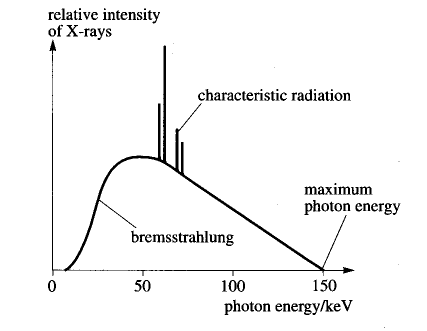
\includegraphics[width=0.7\linewidth]{bramSpec}
	\caption{Bremsstrahalung Spectrum}
	\label{fig:ct:brem}
\end{figure}

\section{Projections and Reconstructions}

The basic equation for taking a projection of an object at a given angle is the following:

\begin{equation}
g(\rho_i,\theta_k) = \int_{-\infty}^{\infty} \int_{-\infty}^{\infty} I(x,y) \; \delta \big(xcos(\theta) + ysin(\theta) - \rho \big) \; dx \; dy
\label{eq:Radon}
\end{equation}
where $g(\rho_i,\theta_k)$ is the radon transform for given sets $\{\rho_i\}$ and $\{\theta_k\}$, $I(x,y)$ is the image that is desired image, or the object, and $\delta$ is the dirac delta function. Back projection then uses these individual projections to create a final image.  For a given $\theta$ the back-projected image is the following:
\begin{equation}
f_{\theta}(x,y) = g(xcos(\theta) + ysin(\theta), \theta)
\end{equation}
Summation of these individual back-projected images generates a final image of the original object:
\begin{equation}
I(x,y) = \sum_{\theta=0}^{\pi} \: f_{\theta}(x,y) = \sum_{\theta=0}^{\pi} \: g(xcos(\theta) + ysin(\theta), \theta)
\end{equation}
However this causes blurring due to multiple projections adding up in the middle (over-sampling), which means that the image obtained is not correct. What is needed is filtered back projection.  A key theorem for this is the central slice theorem which states that the 1-D Fourier transform of a radon transform is a single slice of the 2-D Fourier transform of the image that passes through the origin at angle $\theta$. To prove this, let us consider a single radon transform at angle $\theta$ and take the 1-D Fourier transform of it:
\begin{equation}
G(w,\theta) = \int_{-\infty}^{\infty} g(\rho,\theta) \: e^{i2\pi  w \rho} \: d\rho
\label{eq:1Dft}
\end{equation}
substituting \ref{eq:Radon} into \ref{eq:1Dft} yeilds the following:
\begin{equation}
G(w,\theta) = \int_{-\infty}^{\infty} \: \biggl[  \int_{-\infty}^{\infty} \int_{-\infty}^{\infty} I(x,y) \; \delta \big(xcos(\theta) + ysin(\theta) - \rho \big) \; dx \; dy  \biggr] \: e^{i2\pi  w \rho} \: d\rho
\end{equation}
rearranging this gives:
\begin{equation}
G(w,\theta) = \int_{-\infty}^{\infty} \int_{-\infty}^{\infty} I(x,y) \: \biggl[ \underbrace{ \int_{-\infty}^{\infty} \delta \big(xcos(\theta) + ysin(\theta) - \rho \big) e^{i2\pi w \rho} \: d\rho} \biggr] \: dx \: dy
\end{equation}
using the properties of the dirac delta, the equation can be simplified:
\begin{equation}
G(w,\theta) = \int_{-\infty}^{\infty} \int_{-\infty}^{\infty} I(x,y)   e^{i2\pi w \big(xcos(\theta) + ysin(\theta) \big)} \: dx \: dy \: = \: F(wcos(\theta),wsin(\theta))
\label{eq:sliceThrm}
\end{equation}
Note that this is the a slice of the 2-D Fourier transform along a line $w$ at angle $\theta$. Let us now look at reconstructing the desired image from the Fourier space:
\begin{equation}
I(x,y) = \int_{-\infty}^{\infty} \int_{-\infty}^{\infty} F(u,v)   e^{i2\pi \big(ux + vy \big)} \: du \: dv 
\end{equation}
Now we can convert this to polar coordinates:
\begin{equation}
I(x,y) = \int_{0}^{2\pi} \int_{-\infty}^{\infty} w \: F(wcos(\theta),wsin(\theta))   e^{i2\pi w\big(xcos(\theta) + ysin(\theta) \big)} \:  dw \: d\theta
\end{equation}
Using the Fourier slice theorm from \ref{eq:sliceThrm} we can write the following:
\begin{equation}
I(x,y) = \int_{0}^{2\pi} \int_{-\infty}^{\infty} w\:  G(w,\theta)  e^{i2\pi w\big(xcos(\theta) + ysin(\theta) \big)} \:  dw \: d\theta
\end{equation}
Here we can note that $G(w,\theta + \pi) = G(-w,\theta)$ so we can write the following:
\begin{equation}
I(x,y) = \int_{0}^{\pi} \int_{-\infty}^{\infty} |w|\: G(w,\theta)  e^{i2\pi w\big(xcos(\theta) + ysin(\theta) \big)} \:  dw \: d\theta
\end{equation}
What this shows is that the desired image needs to have the 1-D Fourier transforms of the projections each filtered by $|w|$ in order properly reconstruct the image. This is called filtered back projection and now that the individual projections have been scaled, the reconstructed image is now correct. 

\section{Sampling Criteria}
Assume that the X-ray beam that we are using to generate the projections has a width lets call $\Delta s$ and that the detector that we are using has a certain distance between detector element centers $\Delta r$.  We can now use these distances to define the sampling criteria for CT. Lets say we had a perfect theoretical projection $p_{\theta}(r)$, which never happens, like shown in row 1 of Figure \ref{fig:ct:samp1}. Because the X-ray beam that we are using to generate this projection has some witdth in the real world, we must convolve our prefect projection with a $rect()$ function that has the same width as the beam. Well this is terrible because the fourier relationship of a $rect()$ function is a $sinc()$ function, which sucks because sinc functions go on forever. Well someone decided to draw this awful relationship and that can be seen in row 2 of Figure \ref{fig:ct:samp1}. Anyways, the first lobe of the $sinc()$ function is at $\frac{1}{\Delta s}$ in the frequency domain and since we convolved in the spatial domain, we have to multiply the $sinc()$ function in the frequency domain, thus making our smoothed projection look like it does in row 3 of Figure \ref{fig:ct:samp1}.

\begin{figure}[ht]
	\centering
	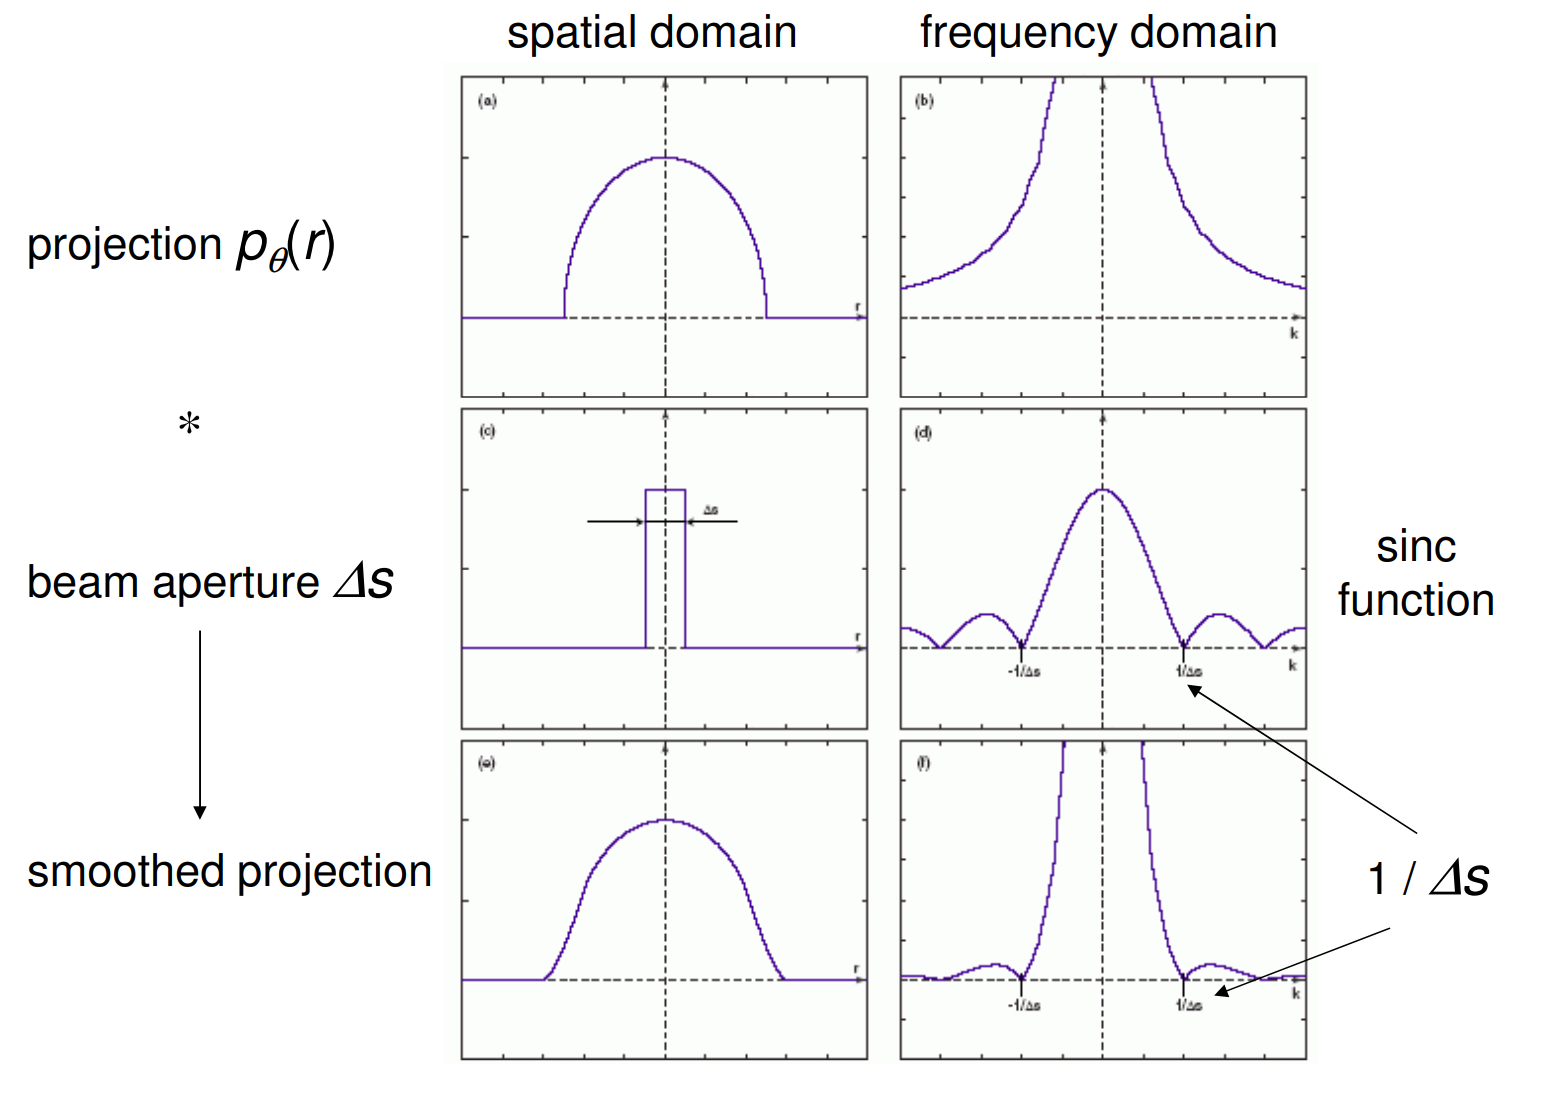
\includegraphics[width=0.9\linewidth]{sampling1}
	\caption{Affect of beam width on projections}
	\label{fig:ct:samp1}
\end{figure}

So remember that Nyquist theory thing? Well it's gonna be important now because if we have samples that are $\Delta r$ apart, which is what we have because that is how far apart our detectors are, then that correlates to $\frac{1}{\Delta r}$ in the frequency domain as can be seen in row 2 of Figure \ref{fig:ct:samp2}. Because we multiply by the sampling function in the spatial domain, we have to convolve in the frequency domain, so our copies can't overlap in the frequency domain. So guess what? No, you are wrong, according to Nyquist, the following must be true so we don't get aliasing:
\begin{equation}
\frac{1}{\Delta r} \leq \frac{2}{\Delta s} \; \; \implies \; \; \Delta r \leq \frac{\Delta s}{2}
\end{equation}
Holy shit! That is at least 2 samples per beam. If this is true, the samples in the frequency domain look like row 3 of Figure \ref{fig:ct:samp2}.
\begin{figure}[ht]
	\centering
	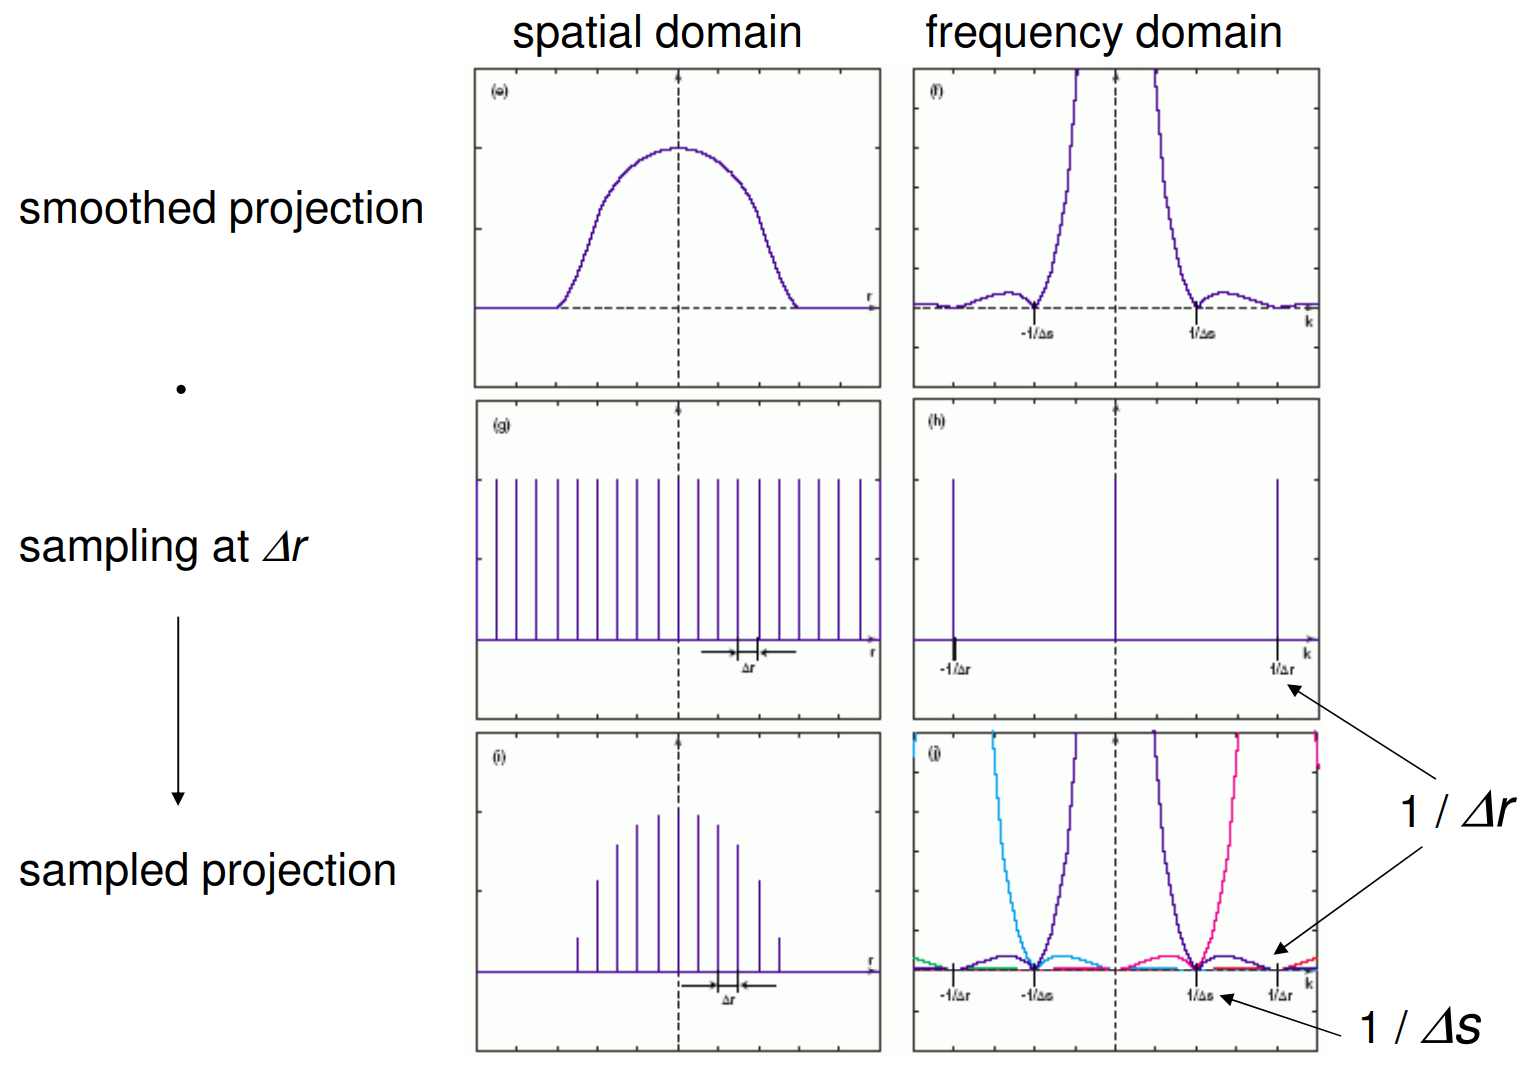
\includegraphics[width=0.9\linewidth]{sampling2}
	\caption{Affect of beam width on projections}
	\label{fig:ct:samp2}
\end{figure}
Now we need to make sure that we get enough different angle projections to get our image back, but what should $\Delta \theta$ be? Well we searched the good old internet and find the "rule of thumb" of CT sampling which is to make the maximum angular sampling the same as the projection sampling ($\Delta \theta = \Delta r$):
\begin{equation}
\Delta \theta = \frac{\pi k_{max}}{M}
\end{equation}
\begin{equation}
\Delta r = \frac{k_{max}}{\frac{N}{2}} 
\end{equation}
\begin{equation}
\Delta \theta = \Delta r \; \; \implies \; \; M = \frac{\pi N}{2}
\end{equation}
where $N$ is the number of detectors, $M$ is the number of radial samples, and $k_{max}$ is the maximum frequency. 

As an example, assume we have the objective to obtain an image with reconstructed resolution of 1mm pixels, with a scanner that has a bank of 512 detectors spaced at 4mm.